\documentclass[aspectratio=169]{beamer}

% Theme selection
\usetheme{Madrid}
\usecolortheme{whale} % Tông xanh đậm chuyên nghiệp cho ngành tài chính

% Packages
\usepackage[utf8]{inputenc}
\usepackage{graphicx}
\usepackage{booktabs}
\usepackage{hyperref}
\usepackage{tikz}
\usepackage{caption}

% Title Slide Info
\title[Personal Finance Management System]{Personal Finance Management System}
\subtitle{Database Management Systems -- Final Project}
\author[Nguyen Phuong Ngan]{Nguyen Phuong Ngan\\ \footnotesize Student ID: 11245914 \and Class: DSEB 66B}
\institute[DSEB 66B]{
    National Economics University \\
    \medskip
    \text{Instructor: PhD. Tran Hung}
}
\date{May 2026}

\begin{document}

% 1. Title Page
\begin{frame}
    \titlepage
\end{frame}

% 2. Agenda
\begin{frame}{Agenda}
    \tableofcontents
\end{frame}

% 3. Problem & Objectives
\section{Problem \& Objectives}
\begin{frame}{Problem Statement \& Objectives}
    \textbf{The Problem:}
    \begin{itemize}
        \item Cash-based transactions in Vietnam make tracking finances difficult.
        \item Lack of structured budgeting leads to missed thresholds and untracked spending patterns.
    \end{itemize}
    
    \vspace{0.3cm}
    \textbf{Project Objectives:}
    \begin{itemize}
        \item Build a persistent, structured relational database using \textbf{MySQL} to enforce business rules.
        \item Deliver an intuitive \textbf{Python-based GUI} (CustomTkinter) for non-technical users.
        \item Automate data integrity (e.g., account balances) via \textbf{Full Lifecycle Triggers}.
        \item Provide actionable visual analytics (income vs. expense, category spending).
    \end{itemize}
\end{frame}

% 4. System Architecture
\section{System Architecture}
\begin{frame}{3-Layer System Architecture}
    The system strictly separates concerns to prevent SQL injection and improve maintainability:
    \vspace{0.2cm}
    
    \begin{itemize}
        \item \textbf{Presentation Layer:} \texttt{main.py} (CustomTkinter). No SQL strings exist here.
        \item \textbf{Business Logic Layer:} \texttt{models.py} + \texttt{reports.py}. Handles parameters and connections.
        \item \textbf{Data Layer:} \textbf{MySQL 8.0}. Executes complex queries and maintains integrity.
    \end{itemize}
    
    \begin{figure}[htbp]
      \centering
      \resizebox{0.8\textwidth}{!}{%
      \begin{tikzpicture}[
        box/.style={rectangle, rounded corners=6pt, draw=structure, fill=structure!10,
                    text width=3.0cm, minimum height=1.2cm, align=center, 
                    font=\small\bfseries, thick},
        arrow/.style={->, >=stealth, thick, color=structure},
        label_font/.style={font=\scriptsize\itshape, color=black!80}
      ]
        \node[box] (ui) at (0,0) {Presentation Layer\\{\footnotesize GUI Screens}};
        \node[box] (bl) at (5,0) {Business Logic Layer\\{\footnotesize models.py}};
        \node[box] (db) at (10,0) {Data Layer\\{\footnotesize MySQL 8.0}};

        \draw[arrow] (ui.east) -- node[midway, above, label_font]{calls} (bl.west);
        \draw[arrow] (bl.east) -- node[midway, above, label_font]{SQL calls} (db.west);
        \draw[arrow] (db.south) -- ++(0,-0.8) -| node[pos=0.25, below, label_font]{Result Sets} (ui.south);
      \end{tikzpicture}%
      }
    \end{figure}
\end{frame}

% 5. Database Design
\section{Database Design}
\begin{frame}{Database Design \& Security}
    \begin{columns}
        \begin{column}{0.45\textwidth}
            \textbf{Core Entities:}
            \begin{itemize}
                \item Users, BankAccounts
                \item Income, Expenses, Categories
                \item Budgets (Monthly Limits)
            \end{itemize}
            \vspace{0.2cm}
            \textbf{Security \& Access Control:}
            \begin{itemize}
                \item \textbf{Restricted User:} \texttt{finance\_app}
                \item \textbf{Least Privilege:} No \texttt{DROP} allowed; \texttt{DELETE} restricted to transactional data only.
                \item \textbf{Integrity:} Balances protected from manual \texttt{UPDATE} (Triggers only).
            \end{itemize}
        \end{column}
        \begin{column}{0.55\textwidth}
            \begin{center}
                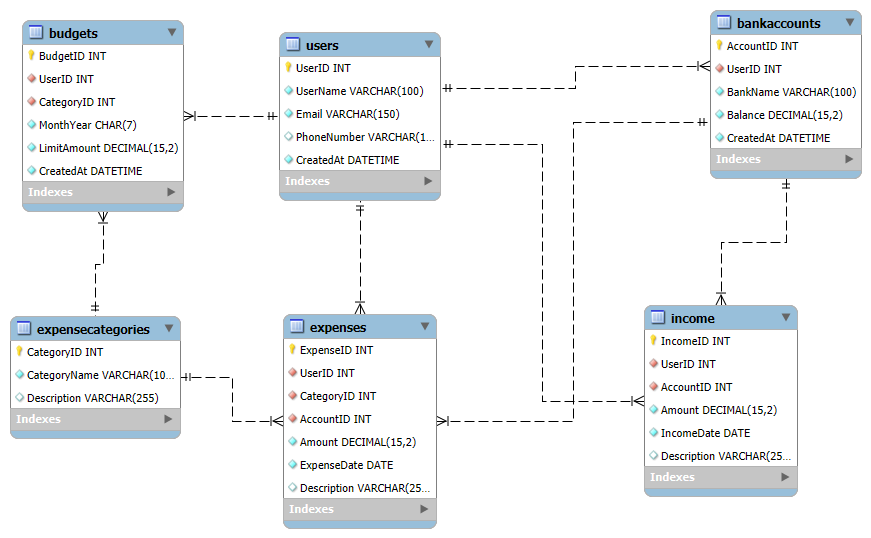
\includegraphics[width=0.9\textwidth]{ERD.png}
                \captionof{figure}{Relational Schema (MySQL)}
            \end{center}
        \end{column}
    \end{columns}
\end{frame}

% 6. Advanced Database Objects
\section{Advanced Database Objects}
\begin{frame}{Advanced Database Objects}
    Business logic is pushed down to the Database Layer for absolute data integrity:
    \vspace{0.2cm}
    \begin{itemize}
        \item \textbf{Full Lifecycle Triggers:} \texttt{AFTER INSERT}, \texttt{UPDATE}, and \texttt{DELETE} on Income/Expenses.
        \begin{itemize}
            \item Automatically restores/adjusts balances even when moving funds between accounts. 
        \end{itemize}
        \item \textbf{Optimized Views:} \texttt{vw\_budget\_status} abstracts complex JOINs and computes usage percentages (OK / WARNING / EXCEEDED).
        \item \textbf{Stored Procedures \& UDFs:} \texttt{sp\_monthly\_report} utilizes \texttt{fn\_total\_expenses} for logic reuse.
        \item \textbf{Indexes:} Composite B-tree indexes on \texttt{(UserID, Date)} for $O(\log n)$ retrieval.
    \end{itemize}
\end{frame}

% 7. Application Implementation
\section{Application Implementation}
\begin{frame}{Python GUI \& Application Screens}
    Built with \textbf{CustomTkinter} and \textbf{Matplotlib}, featuring 4 main modules:
    \vspace{0.2cm}
    \begin{columns}
        \begin{column}{0.55\textwidth}
            \begin{itemize}
                \item \textbf{Dashboard:} Real-time KPI cards and budget alerts.
                \item \textbf{Transactions (CRUD):} Modal Popups for Edit/Delete with DB synchronization.
                \item \textbf{Budgets:} Interactive table with \textbf{In-line Deletion (Trash Icon)}.
                \item \textbf{Reports:} Visualized charts (Bar, Pie, Line trends) with instant refresh logic.
            \end{itemize}
        \end{column}
        \begin{column}{0.45\textwidth}
            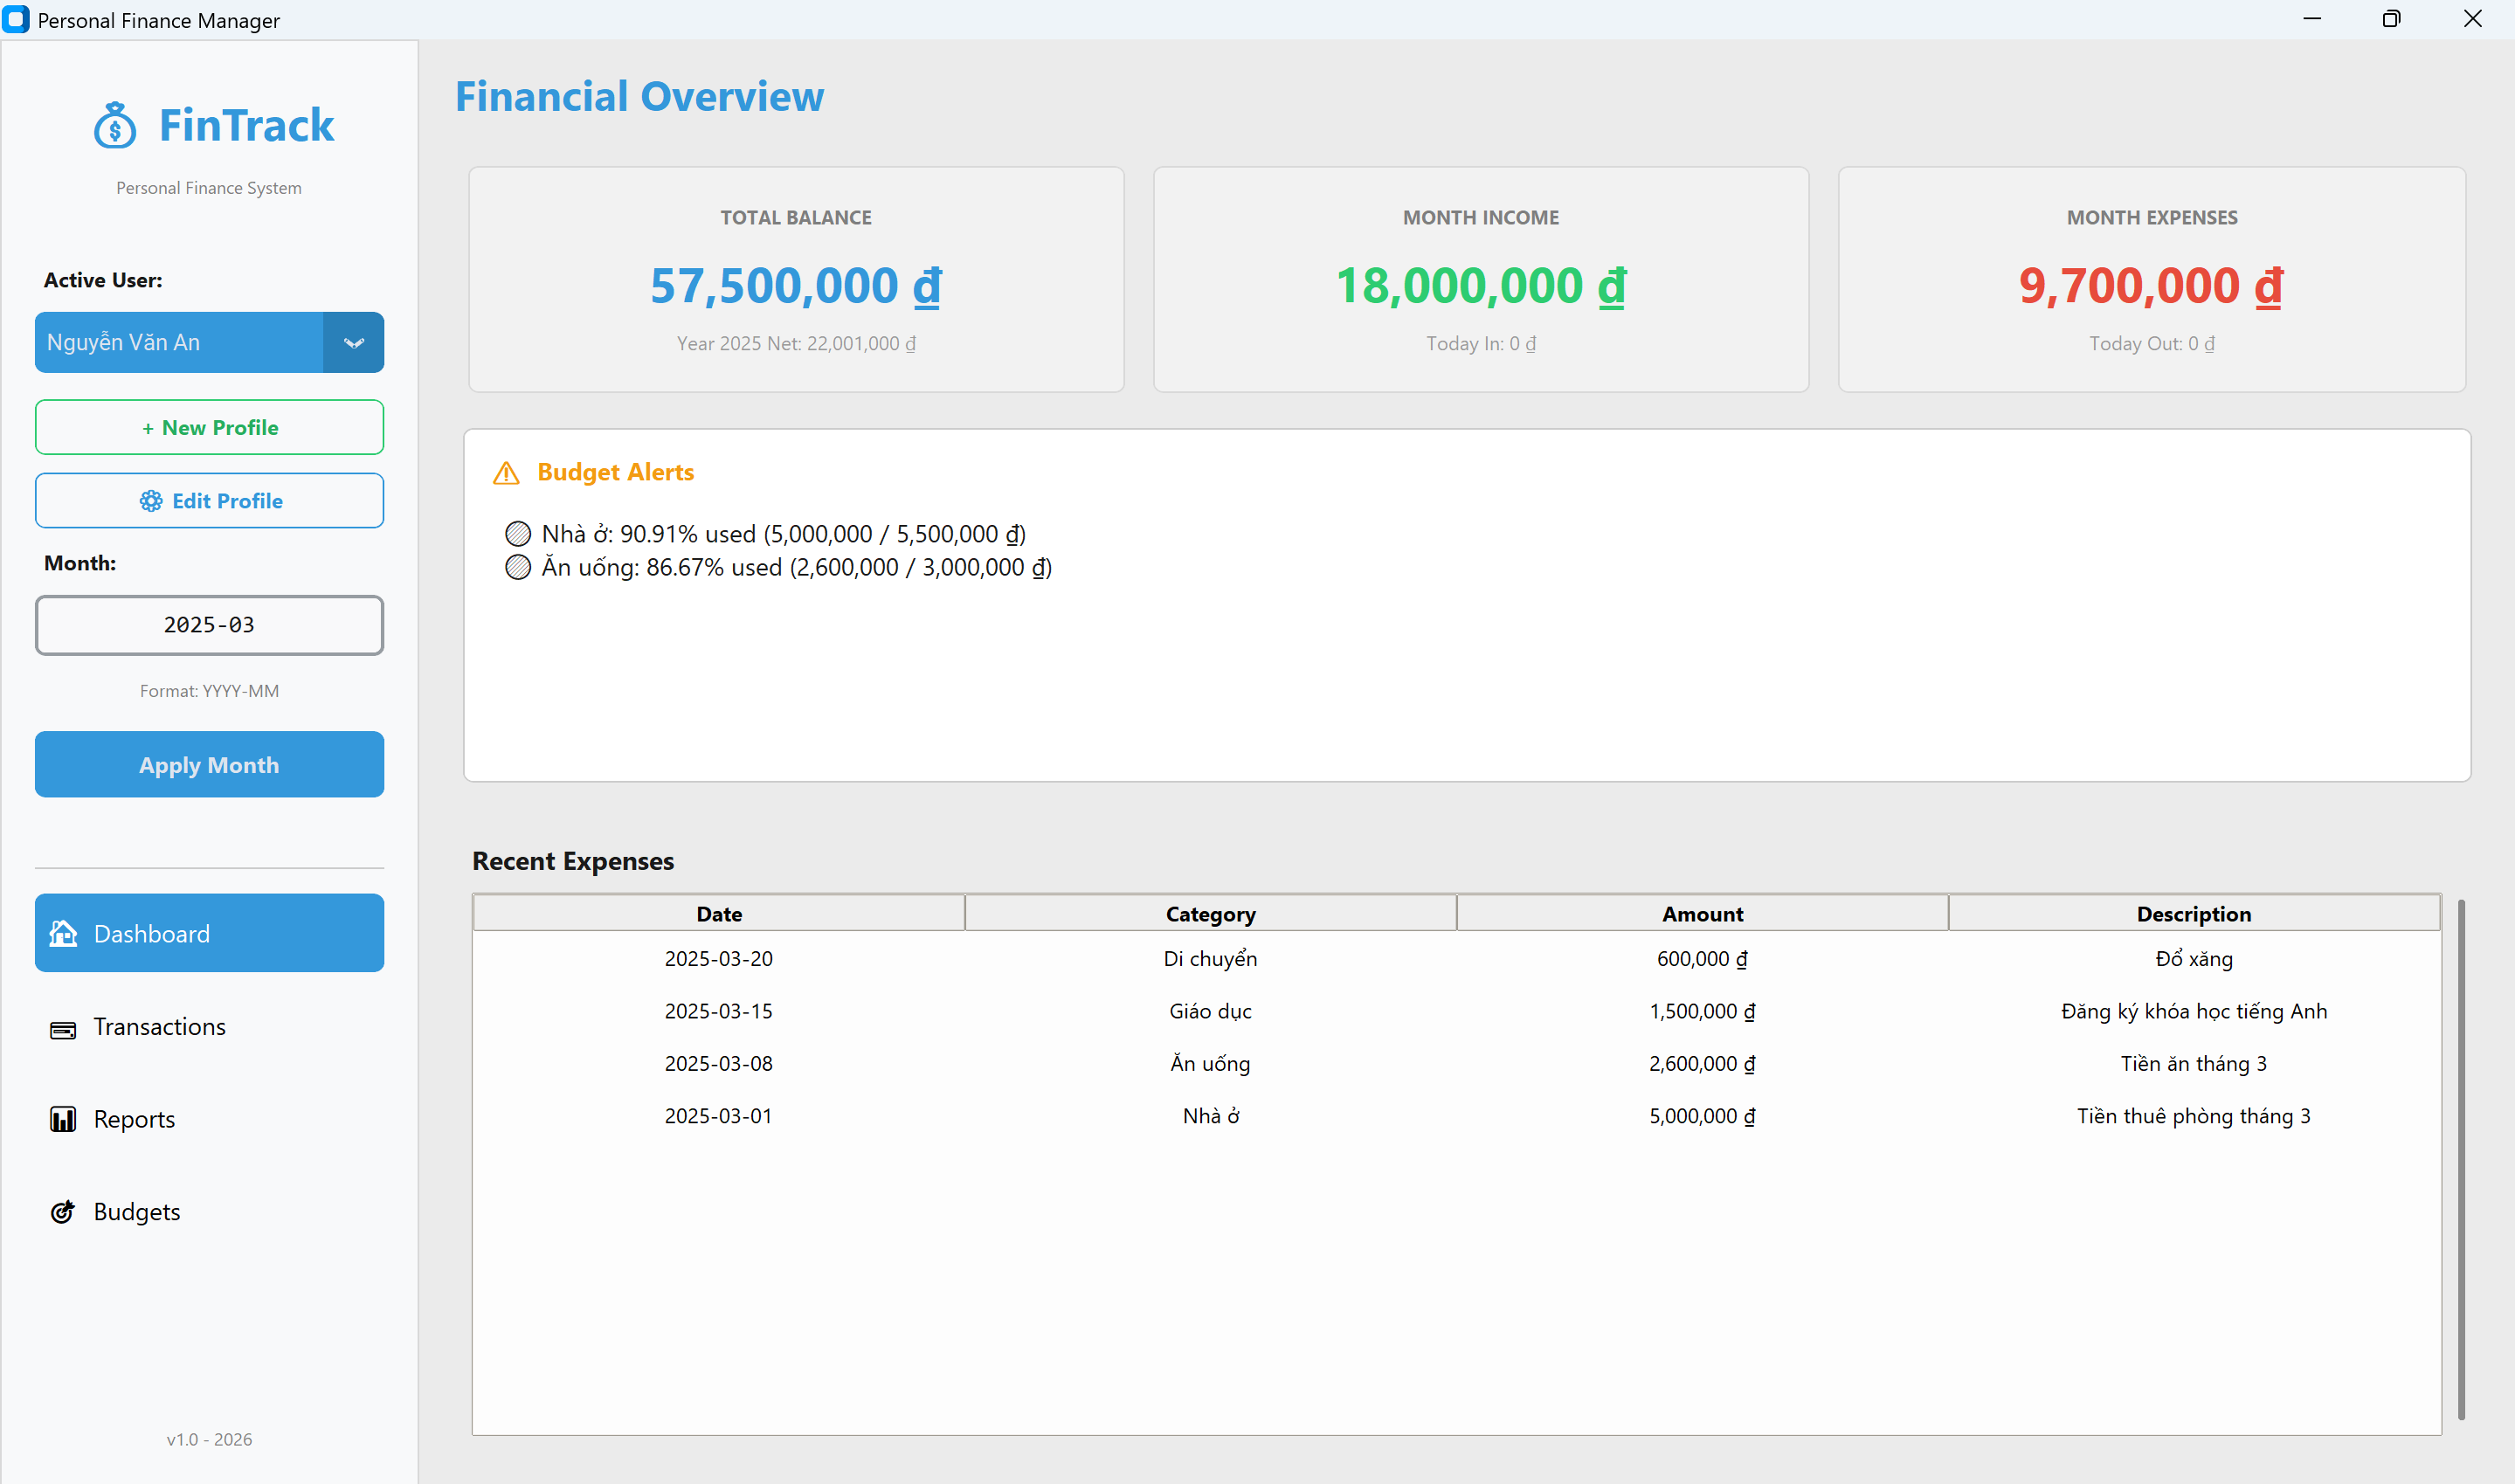
\includegraphics[width=\textwidth]{screenshot/dashboard.png}
        \end{column}
    \end{columns}
\end{frame}

% 8. Conclusion
\section{Conclusion}
\begin{frame}{Conclusion}
    \textbf{Key Achievements:}
    \begin{itemize}
        \item Delivered a fully functional tracking system meeting NEU requirements.
        \item Successfully enforced business invariants reliably using MySQL Triggers.
        \item Implemented a clean, secure 3-layer architecture protecting the DB.
    \end{itemize}
    \vspace{0.4cm}
    \textbf{Future Improvements:}
    \begin{itemize}
        \item Integration with Exchange Rate APIs for multi-currency.
        \item Predictive analytics for budget overrun warnings.
        \item Automated PDF report exports.
    \end{itemize}
\end{frame}

% 9. Q&A
\begin{frame}
    \begin{center}
        \Huge \textbf{Thank you for your attention!}
        
        \vspace{0.5cm}
        \large Demonstration \& Q\&A
    \end{center}
\end{frame}

\end{document}